\documentclass[11pt]{scrartcl}

\usepackage[T1]{fontenc}
\usepackage[utf8]{inputenc}
\usepackage{lmodern}
\usepackage[english]{babel}
\usepackage{xcolor}
\usepackage{amsmath}
\usepackage{amssymb}
\usepackage{amsfonts}
\usepackage{amsthm}
\usepackage[centerdot]{mathtools}
\usepackage{hyperref}
\usepackage{tikz}
\usepackage[ruled]{algorithm2e}
\SetKw{Continue}{continue}
\SetKw{Null}{null}
\SetKw{Break}{break}
\usepackage[textsize=tiny]{todonotes}
\usepackage[normalem]{ulem}
\usepackage{float}
\usepackage{subfig}
\usepackage{pgfplots}
\usepackage{booktabs,caption}
\usepackage[flushleft]{threeparttable}

\newcommand{\daniel}[1]{\todo[linecolor=blue,backgroundcolor=blue!25]{#1}}
\newcommand{\david}[1]{\todo[linecolor=orange,backgroundcolor=orange!25]{#1}}
\newcommand{\laura}[1]{\todo[linecolor=green,backgroundcolor=green!25]{#1}}
\newcommand{\moritz}[1]{\todo[linecolor=red,backgroundcolor=red!25]{#1}}
\newcommand{\changedByLP}[1]{\textcolor{green!50!black}{#1}}
\newcommand{\changedByDP}[1]{\textcolor{blue!50!black}{#1}}
\newcommand{\changedByDK}[1]{\textcolor{orange!50!black}{#1}}
\newcommand{\changedByMW}[1]{\textcolor{red!50!black}{#1}}

\DeclareMathOperator{\cost}{cost}

%\numberwithin{equation}{section}
\newtheorem{theorem}{Theorem}[section]
\newtheorem{lemma}[theorem]{Lemma}
\newtheorem{definition}[theorem]{Definition}
\newtheorem{property}[theorem]{Property}

\title{Optimizing the allocation of vehicles for a Car  Sharing System}
%alternative: The all optimal integer flow problem and its applications.
\author{ Moritz Wegener  7378345}  % in alphabetical order
%\keywords{All integer optimal flow problem; networkflow; minimum cost flow problem}


\begin{document}

\renewcommand{\labelenumi}{\alph{enumi})}		

\date{\today}

\maketitle   
% ist eine vorgegebene Funktion von Latex, die die Variablen automatisch % setzt, automatisch generierte Titelseite

%Logo der Universität zu Köln
{\centering
	
\includegraphics[scale =0.1]{Universitaet_zu_Koeln-Siegel.jpg}
	
	\vspace{2cm}
	\begin{center}
		Faculty of Management, Economics and Social Science \\
		Seminar für Supply Chain Management \& Management Science \\
		University of Cologne \\
		
	\end{center}
	
	
	%keine Seitennummerierung
	\thispagestyle{empty}
	
	
	
	
	%Seite frei
	
}

\newpage
\thispagestyle{empty}
\quad
\newpage
\thispagestyle{empty}

\author{ Moritz Wegener  } 


\maketitle

\begin{abstract} 
This survey presents a stochastic optimization framework to solve the dynamic vehicle allocation problem. The car-sharing service provider needs to manage and determine the optimal number of vehicles at each location at every time in every area. In every time period he has to decide how many cars he wants to rent to customers and how many cars he wants to relocate. The service provider does not know the demand in each period, so the demand is uncertain for him. A multistage stochastic linear programming with uncertain demand is formulated to solve the problem and a numerical example is created and solved.
\end{abstract}

 %Section1 Introduction
\section{Introduction}
Car Sharing is a fast-growing model in the mobility sector. Nearly in every big city in the world, a car-sharing service is offered. It allows members to use private cars without owning an own car \cite{Bardhi_1}. This reduces the costs for the customers and makes the mobility sector more sustainable. People can profit from the benefits of using an own car without bearing the costs of owning one. In 1987, the first car-sharing company was launched in Switzerland. Over the last 30 years, this has developed into a model that is used all over the world \cite{Sus_1}. Generally, car-sharing can be split into two types: reservation-based and free-floating. In the case of reservation-based, customers have to reserve the vehicles before using them, and in the case of free-floating-base, customers can pick up any available car and can directly use it. The rentals of the cars are split into two categories: one-way and round-trip rentals. The difference is that for round trip rentals, the customer has to rent and return the car at the same location. For one-way rentals, rent and return location can be different \cite{Yu_1}.\\
The main impact area of car sharing are transportation, environment, land use, and society \cite{Sus_1}. It brings advantages to all these areas. Some of the major advantages are the following:
\begin{itemize}
\item The reduction of personal transportation costs, because people only pay for the time they rent the car.\cite{Sus_2}
\item The reduction of total traffic, because car-sharing users plan their trips more efficiently. \cite{Cooper_1}
\item A side effect of the traffic reduction is an increase in traffic safety because there are fewer accidents. \cite{Cooper_1}
\item Carsharing leads to a reduction in vehicle ownership and the total number of vehicles.\cite{MACEDO2017731}
\item Many car-sharing service providers use low emission vehicles, which are more sustainable, and people who get a car-sharing membership report to raise a higher awareness for the environment after they get the membership.\cite{Sus_2,lane_1}
\end{itemize}
A big problem that car-sharing service providers face is optimal vehicle allocation. The object is to optimize the vehicle allocation in time and space and maximize the provider's profit. Supply and demand are not always equal in some areas, so the service provider has to reallocate empty vehicles to achieve optimal use of all resources. There are different approaches to solve the problem Fan\cite{Wei_1} discussed a multistage stochastic linear programming model with uncertain demand for one-way reservation-based service. In this survey, the model gets expanded with penalty costs for unfulfilled demand to get a more realistic model.\\
The rest of the survey is structured as follows. First, the problem and assumptions are described. Then the generation of the scenario tree of the uncertain demand is shown. After this, the stochastic programming model is formulated. Based on that, a small case study is presented and solved. The last part is the conclusion, where the results are summarized, and future research opportunities are identified.
\section{Problem Description}
The dynamic vehicle allocation problem can be described as follows. A car-sharing service provider has a given number of vehicles and wants to offer his service at a given number of locations in the neighborhood for a time horizon. The customer can rent a car and drive from one place to the same or another location. The service provider can reallocate all vehicles that customers do not use. At the beginning of a time horizon, the service provider knows the number of customers who want to rent a car and drive from one specific to another specific location. He has to decide if he wants to accept each customer's reservation or if he wants to reject the reservation, e.g., if the reservation is unprofitable or if he is unable to fulfill the total demand. Also, he has to decide how to allocate the vehicles, which the customers do not use. For every accepted reservation, he gets a revenue, for every rejected reservation, he gets penalty costs, and for every reallocation, he has to pay a given price.
The car-sharing service manager has to decide at the beginning of every period how many reservations he wants to accept, how many he wants to reject, and how he wants to reallocate the vehicles.
The manager only knows the demand for the current period, but not for the future periods, so the demand is uncertain for him.\\
He aims to maximize the total profit over N periods by using independent random future demands with a known distribution. The increasing level of future uncertainty makes this problem a difficult stochastic problem. To model the problem, the following assumptions are made: (1) The time is measured in intervals or periods (in this case one day); in each period, every vehicle is assigned to a customer, is moved empty to another location or stays at the location. (2) The customers make reservations for the next period at the end of each period, so the car-sharing service provider knows the demand at the beginning of each period. (3) The vehicles are picked up at a specific location. (4) The cars are dropped off at any car-sharing location at a particular time the following day. (5) Customers can not share vehicles to fulfill their demand during a period, so each customer needs one car for the whole period two satisfy his demand. (6) A journey between two locations lasts one day. (7) All unfulfilled demands during a period are lost and penalized with costs. (8) All cars are available in the first period. (9) The mean values and the distribution for the demand between two locations are known, and it is assumed to be discrete.\\
We can now formulate this as a profit-maximization problem and develop a stochastic model.
\section{Scenario Generation}
\label{Scenario}
The scenarios that represent the demand uncertainty and are used to solve the problem are generated with a discrete distribution. The demand for the first period is known and decisions are made based on the information, so for the first-period uncertainty does not matter. In every other period the demand can be low, medium, or high. In Figure \ref{fig:scenarios} a scenario tree for the first two periods is presented.
Every node in the tree represents the state in period t, and every arc the realizations of the uncertain demand. The decision the car-sharing service manager has to make depends on the decision he has made in the periods before the current state and the uncurtained demands in the current period. In the real-world only the solution of the first stage will be used to make a decision. The decisions after the first stage are only made to calculate the first-stage decisions \cite{FLETEN200237}.
\begin{figure}[H]
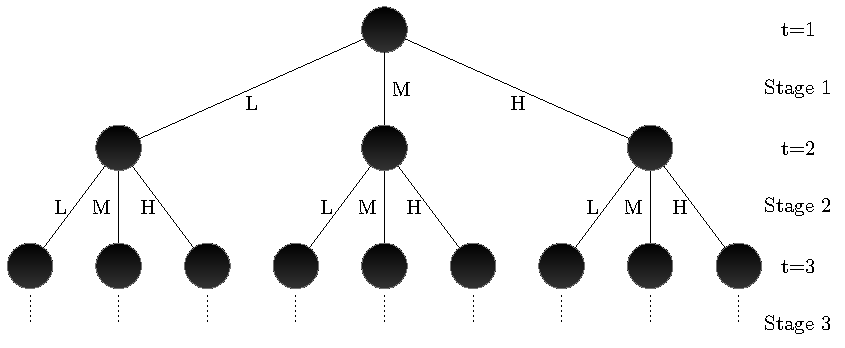
\includegraphics{Figures/figure.pdf}
\caption{Scenario tree based on \cite{Wei_1}. L = low demand, M = medium demand, H = high demand }
\centering
\label{fig:scenarios}
\end{figure}
At the beginning of the first period the manager makes a decision based on the information he gets. He sees the consequences in the next period and gains new information from that. Based on this information and the demand distribution he makes decisions in the second period for the third period. The same process is then used for the other periods as well. For each scenario tree the optimal solution can be determined. The number of scenarios is given by $\Omega^{T-1}$.

\section{Model formulation}
In the first part all random distributions, parameters, data, and decision variables necessary to solve the optimization problem are presented. After this the objective function and explain all constraints are shown. The result is a stochastic programming model for a planning horizon of $N$ day.
\subsection{Notation}
The following notations are used in the model.
\begin{description}
\item[Indices:] ~\par

\textbf{$i , j \in R$} = locations to pickup or drop of cars.\\
$t \in T$ = a periode in the planing horizion.\\
$\omega \in \Omega $ = scenarios.
\end{description}
\begin{description}
\item[Parameters and data:] ~\par
$r_{i j}=$ revenue for a fullfiled demand from start location $i$ to end location $j$.\\
$c_{i j}=$ cost of reallocating a car from start location $i$ to end location $j$.\\
$r_{i j}=$ net revenue for satisfying a carsharing demand from start location $i$ to end location $j$.\\
$o_{i j}=$ penalty cost for unfullfield demand from start location $i$ to end location $j$.\\
$L_{i j 1}=$ number of requests by custemors in the first period $(t=1)$ to be available to move from start location $i$ to end location $j$.\\
$d_{i j t}^{\omega}=$ number of customers that need a car to drive from start location $i$ to end location $j$ during period $t$ in scenario $\omega, t=2, \ldots, N $ .\\
$S_{i 1}=$ number of vehicles at location $i$ at the beginning of period 1.\\
$p^{\omega} = $ Probability of scenario $\omega$.
\end{description}
\begin{description}
\item[Random distributions:] ~\par
$\tilde{d}_{i j t}=$ random demand that denotes the number of customers needing transportation from start location $i$ to end location $j$ during period $t, t=2, \ldots, N ;$
\end{description}
\begin{description}
\item[Decision variables:] ~\par
$x_{i j t}^{\omega}=$ number of vehicles that are used by customers to drive from start location $i$ to end location $j$ in period $t$ in scenario $w, t=1,2, \ldots, N ;$\\
$y_{i j t}^{\omega}=$ number of vehicles that are reallocated from start location $i$ to location $j$ in period $t$ in scenario $w, t=1,$ $2, \ldots, N$\\
$S_{i t}^{\omega}=$ number of vehicles at location $i$ at the beginning of period $t$ in scenario $w, t=2, \ldots, N$\\
$z_{i j t}^{\omega}=$ number of vehicle reservations that got cancelled from start location $i$ to end location $j$ in period $t$ in scenario $w, t=1,$ $2, \ldots, N$\\
\end{description}
\subsection{Penalty Cost}
Penalty costs for a risk-neutral service provider are added to the model by \cite{Wei_1}. The penalty costs represent costs for the unmet demand. This factor is quite important because unmet demand plays a huge role in the mobility sector. If a car-sharing service provider rejects customers' reservations on their first trip or multiple times, the customer probably will not use the service again. This could not only influence the relationship between this specific customer and the car-sharing provider. If the customer shares his opinion with other possible customers, e.g., via social media, it could also influence the other possible customers and the brand image. Over the longer term, this could reduce the number of customers and reservation requests because customers will use more reliable services that have a better image. This leads to costs for the service provider.\\
There are different ways to model the penalty costs. If the model should deal with uncertainty penalty costs, the costs must be part of the scenarios, and the distribution of the costs must be determined. The major problem is that this increases the scenario size and makes the calculation way more complex for a huge number of periods. That is why this approach is rejected. Another option is to set constant costs for every unmet demand independent of the start and end location. This is a very easy way and can be the right approach if unmet demand damage is the same at every location. If the cost of unmet demand depends on the area, every possible combination of start and end location needs its own cost for every unmet demand. In the case studie both options are solved and the solutions are compared. A factor that influences the penalty costs in a hughe way is the number of mobility competitors and alternative traveling options. If the number of competitors is very high, the penalty costs should be high because then customers have a lot of other travel options. On the other side, if there is no competitor, the penalty costs should also be high because the customers have no other option to travel. The risk, in this case, is that he will stop using public transportation and use a private car instead. So the costs should be low if the competition is not very high, but the customer still has other publication transport options to travel with if his reservation gets canceled.
\subsection{Model}
The optimization model for each period $t=1,2, \ldots, N ;$\\
\begin{equation}
h(x_{i j}^{\omega},y_{i j t}^{\omega},z_{i j t}^{\omega},d_{i j t}^{\omega}) = {Max }_{x_{i j t}^{\omega},y_{i j t}^{\omega},z_{i j t}^{\omega}}\sum_{i=1}^{R} \sum_{j=1}^{R} \sum_{t=1}^{T} \sum_{\omega=1}^{\Omega}(x_{i j t}^{\omega}\cdot r_{i j} - y_{i j t}^{\omega} \cdot c_{i j} - z_{i j t}^{\omega} \cdot o_{i j})\cdot p^{\omega}
\end{equation}
\begin{align}
x_{i j 1}^{\omega} \leq L_{i j 1} & & i \in R ; j \in R \\
x_{i j t}^{\omega} \leq d_{i j t}^{\omega} & & i \in R ; j \in R ; t=2,3, \ldots, N ; \omega \in \Omega \\
z_{i j t}^{\omega} - x_{i j t}^{\omega} = d_{i j t}^{\omega} \\
z_{i j 1}^{\omega} - x_{i j 1}^{\omega} = L_{i j 1} \\
\sum_{j}\left(x_{i j t}^{\omega}+y_{i j t}^{\omega}\right)=S_{i t}^{\omega} & & i \in R ; t=2,3, \ldots, N ; \omega \in \Omega \\
\sum_{j}\left(x_{i j 1}^{\omega}+y_{i j 1}^{\omega}\right)=S_{i 1} & & i \in R ; \omega \in \Omega \\
\sum_{i}\left(x_{i j t}^{\omega}+y_{i j t}^{\omega}\right)=S_{j(t+1)}^{\omega} & & j \in R ; t=1,2, \ldots, N-1\\
x_{i j t}^{\omega}, y_{i j t}^{\omega}, S_{i t}^{\omega},z_{i j 1}^{\omega}, \geq 0 & & i \in R ; j \in R ; t=1,2, \ldots, N ; \omega \in \Omega\\
x_{i j t}^{\omega}, y_{i j t}^{\omega}, S_{i t}^{\omega},z_{i j 1}^{\omega}, \text { must be integers } & & i \in R ; j \in R ; t=1,2, \ldots, N ; \omega \in \Omega
\end{align}
\\
The objective function is to maximize the profit of the model. The profit is calculated by multiplying the number of vehicles that are used by costumes with the revenue. From this value, all reallocation and penalty costs are subtracted. Constraint (1) and (2) state that the number of customers who drive a car from a location to another location in each period must be smaller or equal to the total demand for this location combination under each scenario. Constraint (3) and (4) say that the number of customers who drive a car from a location to another location plus the number of customers which reservation is canceled for the same location combination must be the same as the total demand for this location combination under each scenario and each period. Constraint (5) and (6) guarantee that the supply of a location can not be exceeded by the number of cars rented by customers and allocated in a period for all scenario. Constraint (8) says that the number of cars that arive at the end of a day at the location must be the same as the number of cars that are available at the next period (for each period and each scenario). The last two conditions (9) and (10) are for nonnegativity and integer properties.\\
We see that this problem is a stochastic linear programming problem because of uncertain demand in the constraints. The problem is that we can deal with an infinite planning horizon, so we have truncated the horizon to a certain number (N). This can cause differences in the optimal solution compared to the infinite time horizon. For a marginal problem size, the problem can get solved with the simplex algorithm.
\section{Case Study}
To solve the problem and test the quality and computation time of the solution a seven-stage network is generated. The model was implemented in the programming language Julia and solved with a cplex solver. It was tested on hardware with 16 GB memory and CPU with four 1.99 GHz cores.
\subsection{Numerical Example}
The matrices with the revenue per drive and the cost for allocation have the following values. Each unit in the matrix represents one dollar.
\\
\begin{equation*}
r_{i j} =
\begin{pmatrix}
10&11& 9& 14\\
12& 15& 10& 9\\
12& 6 & 7 &9\\
14 &12 &10& 8
\end{pmatrix}
\quad
c_{i j} =
\begin{pmatrix}
0& 3& 4& 4\\
3 &0 &4 &5\\
4 &4& 0& 6\\
4& 5& 6& 0\\
\end{pmatrix}
\end{equation*}
\\
In $t=1$ the demands for rides between each location pair and the number of vehicles located at each starting position are fixed and have the following value.
\begin{equation*}
L_{i j 1} =
\begin{pmatrix}
25 &20& 23& 16\\
18& 23& 22& 21\\
17&25& 19& 26\\
19&25& 27& 16
\end{pmatrix}
\quad
S_{i,1}=
\begin{pmatrix}
90\\
100\\
90\\
90\\
\end{pmatrix}
\end{equation*}
\\
The following four matrixes describe the demand distribution. For each possible demand (low medium and high) is represented by a matrix $d_{i j t}^{\omega}$. The possibility for low demand is 40\%, medium demand is 20\%, and high demand is 40\%. Based on the matrices and the probabilities, the average demand for each location pair is calculated and shown in matrix $d_{i,j,k}$.
\\
\begin{equation*}
p^{low} = 0.4\\
\end{equation*}
\begin{equation*}
p^{medium} = 0.2\\
\end{equation*}
\begin{equation*}
p^{high} = 0.4\\
\end{equation*}

\begin{equation*}
d_{i j t}^{low} =
\begin{pmatrix}
17& 12& 15& 12\\
9 &13& 10& 10\\
6 &15 &17 &11\\
10 &17& 21 &15\\
\end{pmatrix}
\quad
d_{i j t}^{medium}
\begin{pmatrix}
26& 21& 24 &13\\
20 &19& 27& 21\\
14 &22 &19& 21\\
17& 26& 27& 20\\
\end{pmatrix}
\end{equation*}
\\
\begin{equation*}
d_{i j t}^{high}
\begin{pmatrix}
40 &35& 38& 29\\
36& 35& 39& 42\\
37 &39& 26 &46\\
29& 40& 48& 30\\
\end{pmatrix}
\quad
d_{i j t}=
\begin{pmatrix}
28&23&26&19\\
22&23&25&25\\
20&26&21&27\\
19&28&33&22\\
\end{pmatrix}
\end{equation*}
\\
To model the penalty cost for unmet demand two possibilities exist in the first case the penalty costs for every location pair has the same value. So for penalty costs of 10 the matrix looks like this:
\\
\begin{equation*}
o_{i j}=
\begin{pmatrix}
10& 10& 10& 10\\
10 &10 &10 &10\\
10&10& 10&10\\
10& 10& 10& 10\\
\end{pmatrix}
\end{equation*}
\\
In the other case penalty costs are individual per location pair. The matrix looks like this:
\begin{equation*}
o_{i j}=
\begin{pmatrix}
15&9&8&7\\
11&14&12&13\\
11&12&9&13\\
17&18&12&15\\
\end{pmatrix}
\end{equation*}
\\
\subsection{Results}
The computition of the model is highly fast, the results were calculated in seconds. The solution of the numerical example in case of same penalty costs for every location pair is shown in Table \ref{tab:results}. The revenue for all penalty costs betwen \$0 and \$80 was calculated. The revenue decreases when the penalty costs increase. The tabel shows that the first negative revenue is for penalty cost of \$50. A more detailed analysis shows that the last positive revenue is at \$44, so until this point the service is profitable. \\
\begin{table}[h]
\centering
\begin{tabular}{c|r}
penalty costs in \$ & revenue in \$\\
\hline
0 & 23,002.21 \\
10 & 17,746.21 \\
20 & 12,490.21 \\
30 & 7,234.21 \\
40 & 1,978.21 \\
50 & -3,277.78 \\
60 & -8,533.78\\
70 & -13,789.78\\
80 & -19,045.78\\
\end{tabular}
\caption{Results}
\label{tab:results}
\end{table}
\\
The result for the example with individual penalty cost is \$16,998.25. The model has a positive revenue and is profitable. The results show that a car service sharing provider can calculate the revenue of his service in this way and can check if his service is lucrative. Other results of the model are the decisions the service provider has to make in stage one. As mentioned in Section~\ref{Scenario}., these are the decisions a provider has to make in the real world. The following matrices show how many reservations the service provider should accept for each location pair and how he should reallocate the other vehicles if he uses individual penalty cost.
\\
\begin{equation*}
x_{i j 1}=
\begin{pmatrix}
25 &20& 23& 16\\
18 &23 &22 &21\\
17& 25& 19& 26\\
19& 25 &27 &16
\end{pmatrix}
\quad
y_{i j 1}=
\begin{pmatrix}
6 &0 &0&0\\
16& 0 &0 &0\\
0 &0 &3 &0\\
0& 0& 0& 3\\
\end{pmatrix}
\end{equation*}

\input{Chapters/Conclusion.tex}
\newpage
 \bibliographystyle{plain}
 \bibliography{libary.bib}


\end{document}

